\documentclass[12pt]{article}

\usepackage{tgtermes}
\usepackage{epsf}
\usepackage{epstopdf}
\usepackage{amsmath}
\usepackage{graphicx}
\usepackage{booktabs}
\usepackage[colorlinks=true,linkcolor=blue,citecolor=blue]{hyperref}
\usepackage{dcolumn}
\usepackage{amsmath, amsthm, amssymb}
\usepackage{mwe}
\usepackage{url}
\usepackage{natbib}
%\usepackage{harvard}
\usepackage{fancyheadings}
\usepackage{longtable}
\usepackage{authblk}
\usepackage{setspace}
%\usepackage[nomarkers]{endfloat}
\usepackage{float}
\usepackage{bbm}
%\usepackage{titling}
\usepackage{subcaption}
\usepackage{algorithm}
\usepackage{algorithmic}
\usepackage{import}
\usepackage[backend=biber,style=authoryear,
sorting=ynt,citestyle=authoryear]{biblatex}
\addbibresource{papercitations.bib}
%\usepackage[nomarkers,nofiglist,notablist]{endfloat}

\onehalfspacing
\textwidth 6.5in \oddsidemargin 0in \evensidemargin -0.6in
\textheight 8.5in \topmargin -0.2in

\newcolumntype{L}[1]{>{\raggedright\let\newline\\
		\arraybackslash\hspace{0pt}}m{#1}}
\newcolumntype{C}[1]{>{\centering\let\newline\\
		\arraybackslash\hspace{0pt}}m{#1}}
\newcolumntype{R}[1]{>{\raggedleft\let\newline\\
		\arraybackslash\hspace{0pt}}m{#1}}
\newcolumntype{P}[1]{>{\raggedright\tabularxbackslash}p{#1}}

\newtheorem{theorem}{Theorem}[section]
\newtheorem{corollary}[theorem]{Corollary}
\newtheorem{proposition}[theorem]{Proposition}
\newtheorem{lemma}[theorem]{Lemma}

\captionsetup{justification=raggedright,singlelinecheck=false}


\newcommand{\xsub}[1]{%
	\mbox{\scriptsize\begin{tabular}{@{}c@{}}#1\end{tabular}}%
}

%\renewcommand{\thetable}{\Roman{table}}

\begin{document}
	
	
	
	
	\linespread{1.2}\title{\vspace{-0.5in} Does Hospital Leadership Matter?\\ \large Evidence from the Hospital Readmissions Reduction Program} 
	
	\date{\today}
	
	\author{\vspace{10mm}Hanna Glenn\footnote{Department of Economics, Emory University, 1602 Fishburne Drive, Atlanta, GA 30322, hanna.glenn@emory.edu.} }
	
	\maketitle
	%\setlength{\droptitle}{-10pt}
	
	\vspace{-0.2in}
	
	\singlespacing\maketitle
	
	\begin{abstract}
		{\small
			
			
		} 
	\end{abstract}
	
	
	
	
	\vspace{0.1in}
	
	\noindent Keywords: 
	
	\noindent JEL Codes: 
	
	\onehalfspacing
	
	\newpage

  The objectives and behaviors of firms that are not classic for-profits are not easily determined, and an extensive literature has sought to understand these types of firms. Nonprofits are thought to gain utility not solely from monetary profit, but also through accomplishing mission-based purposes. Researchers have speculated a variety of objective functions that could motivate nonprofits such as maximizing prestige, income, or a quality/quantity tradeoff (Steinberg, 1986). An important contribution to this literature is the use of empirical strategies to analyze how firm behavior reveals attributes of the underlying objective function (add citations). In this paper, I leverage a large-scale shock to nonprofit hospitals in the US to investigate whether characteristics of the objective function is revealed by the composition of their leadership team.
  
  Hospitals in particular have been a common focus when seeking to understand not-for-profit firms. This is because, first, there are different hospital ownership types within the industry, giving researchers the ability to compare the behaviors of nonprofits with that of for-profits. Second, nonprofit hospitals make up over 50\% of all hospitals in the US, and staff, on average, 207 beds. For comparison, for-profits make up around 36\% of hospitals and staff 107 beds (\cite{ASPE_2023}). Thus, nonprofit behavior in the hospital industry is relevant and directly affects consumers of health care. However, it remains unclear what type of objective function drives nonprofit hospitals (Erus \& Weisbrod, 2002; Deneffee \& Masson, 2002; Horwitz \& Nichols, 2009). 
  
  What has not been considered is how the leadership team within nonprofits potentially drives objectives. In large, publicly traded firms, executive characteristics are shown to be correlated with firm performance, indicating that there is more to firm behavior than just for-profit or not-for-profit status. Within nonprofit hospitals, there is variation in the propensity to hire executives with a background in clinical work, which could reasonably change how much weight the hospital places on profit vs. quality of care in their objective function. I contribute to our understanding of hospital and nonprofit behaviors by investigating whether clinical experience on an executive team affects hospital behavior after being financially penalized.

  Using publicly available tax forms, I construct a novel data set of nonprofit hospitals from 2009-2015 which captures the identities of executives tied to that hospital. I link hospitals in this data to hospital level characteristics in the American Hospital Association survey and Hospital Compare data. In order to capture the effect of clinical experience in executives, not just the selection of clinical executives into certain types of hospitals, I specifically investigate hospitals penalized by the Hospital Readmissions Reduction Program (HRRP) of 2012. This program reduced Medicare payments to hospitals with above average readmission rates, and is plausibly uncorrelated with previously determined leadership teams. I further limit the sample to hospitals with stable executive teams over time, and characterize hospitals as having clinical experience on their team or not. I estimate the difference in readmission and mortality rates between hospitals with and without clinical experience before and after the penalties began, conditional on being penalized. I assume that before the penalty, clinical and non-clinical team hospitals had similar readmission and mortality trends, and that the composition of hospital executive teams determined prior to the penalties is, conditional on being penalized, exogenous. Under these assumptions, I identify the effect of having a clinical executive on a hospital’s response to the penalty measured in readmission and mortality rates. 

    I find that

    I contribute to hospital objectives

    I contribute to HRRP

    I contribute to executives affect on firms

    

    \section{Background}

    \subsection{Hospital Readmissions Reduction Program}

    A readmission is when a patient returns to the hospital within 30 days of being discharged from a previous stay; avoidable readmissions are a bad outcome for patients and increase health care spending. The Hospital Readmissions Reduction Program (HRRP) was enacted in 2010 as a part of the Affordable Care Act to incentivize hospitals to reduce readmission rates. The goal of the program was to get hospitals to lower readmissions through better care coordination, less initial stay complications, and better post-care instructions. Beginning in October 2012, hospitals with higher readmission rates than the national average in pneumonia, heart failure, or AMI (after adjusting for demographic characteristics faced by the hospital) receive a lower reimbursement rate for all Medicare patients they treat. The penalties are based on each hospital's past performance in readmissions, which means hospitals had incentive to react immediately once details of the program were announced in October of 2011. 

    \subsection{Nonprofit Hospital Leadership}

    Nonprofits are governed by a board of directors, whose role is to set high level goals and strategies, and provide general oversight. The board is not in charge of day-to-day operations, but the general direction of the firm. They select members of the executive team to carry out day-to-day operations. The executive team usually consists of at least a CEO and CFO. Every nonprofit is different in exactly how they structure an executive team. Some nonprofits hire Chief Medical Officers, Chief Quality Officers, executive directors, vice presidents of various departments, etc. I consider all of these employees as part of the day-to-day management of the hospital and include them in the executive team. 

  
	
	\section{Data}\label{sec:data}

    \subsection{Names of Hospital Leaders}

    To characterize hospitals as having clinical experience on executive team or not, I construct a novel data set of nonprofit hospitals in the US which contains names and select characteristics of executives tied to the hospital from 2009-2015. I gather this data from each hospital's publicly available Tax Form 990, which is required each year for all nonprofits in the US. To my knowledge, this is the first large scale gathering of leadership names from these forms. I include a very detailed account of the collection of this data in Appendix \ref{appendixdata}.

    The tax forms for all nonprofits are housed by ProPublica\footnote{https://projects.propublica.org/nonprofits/}. I use the NonProfit Explorer API to extract the Employee Identification Numbers (EIN) of all nonprofits classified as a hospital according to their National Taxonomy of Exempt Entities (NTEE) code. After filtering out associations and specialty hospitals, there are around 3000 nonprofit hospitals left. Importantly, I need to be able to link EINs to other hospital characteristics, including penalty status and readmission/mortality rates, in the American Hospital Association annual survey and Hospital Compare data. No official crosswalk between the two identification methods exists, so I must rely on matching via location and name of hospital in both data sets. After limiting to only general, nonprofit hospitals in AHA, I confidently match approximately 1200 EINs to an AHA identification number based on exact name matches within the same state. 
    
    For each of the 1200 EINs, I extract urls to 990 pdfs in each year. I download these locally and use OCR text extraction methods to scrape the relevant section of the pdf, which is titled ``Officers, Directors, Trustees, Key Employees, and Highest Compensated Employees". Finally, I use string cleaning methods to identify names and positions for each EIN, year. I also identify titles indicating the person is a physician: md, dr., or do. Using OCR extraction can be unreliable in some instances where the text is handwritten or the font is too small. Therefore, I manually find names, positions, and titles for observations that are missing after the initial extraction.

    My identification strategy relies on hospitals which have stable executive leadership characteristics over time. The ideal sample would be hospitals who have the same people on their team for the entire sample. However, this rarely occurs in reality. Therefore, I proxy for a stable leadership in two ways. First, since my main focus is clinical experience, I limit the sample to hospitals who do not change the presence of a doctor on their leadership team from 2010-2014. Second, I increase the restriction by limiting the sample again to those also who do not change their CEO from 2010-2014. Finally, I aggregate the information up to the hospital level, where an observation captures whether the hospital has clinical experience on their executive team over the course of the sample. 


    \subsection{Other Hospital Characteristics and Outcomes}

    I merge this hospital-level data with the American Hospital Association (AHA) survey using the EIN-AHA links I created based on hospital names. From AHA, I gather the number of beds in the hospital and the Medicare number, which I use to merge in the Hospital Compare data. Hospital Compare contains multiple data sets which I use to identify hospitals that were penalized in the Hospital Readmissions Reduction Program (HRRP), along with yearly readmission and mortality rates for the relevant HRRP conditions: heart failure, heart attack, and pneumonia, my outcomes of interest.

    The Hospital Compare excess readmissions files contain hospital level information on the excess readmission measure used by CMS to determine whether a hospital should be penalized. This variable is also condition specific, where a hospital is penalized if any of the three excess readmission ratios are greater than one. Further, Hospital Compare also publishes hospital level readmission and mortality rates for heart failure, heart attack, and pneumonia. For my main outcomes of interest, I take an average across conditions and weight it using the total number of patients in that condition. For further analysis, I create samples of hospitals who were penalized for specific conditions and investigate the change in readmission and mortality rates for the condition they were penalized for. 

    \import{Tables}{noMDchg_sumstats.tex}

    Figure \ref{weighted_read_mort_graph} shows the average of the main outcomes across all penalized hospitals over time. While mortality rates did not seem to change much after the penalties began in 2012, readmission rates decreased after the penalty for hospitals with and without clinical experience. However, readmission rates for non-clinical hospitals decreased more dramatically than those for clinical hospitals, even dropping below those for clinical teams in 2013 and 2014. While suggestive, this motivates further analysis into the differential responses between clinical and non-clinical research teams. 

    \begin{figure}[h!]
        \centering
        \caption{Readmission rates over time in all penalized hospitals}
        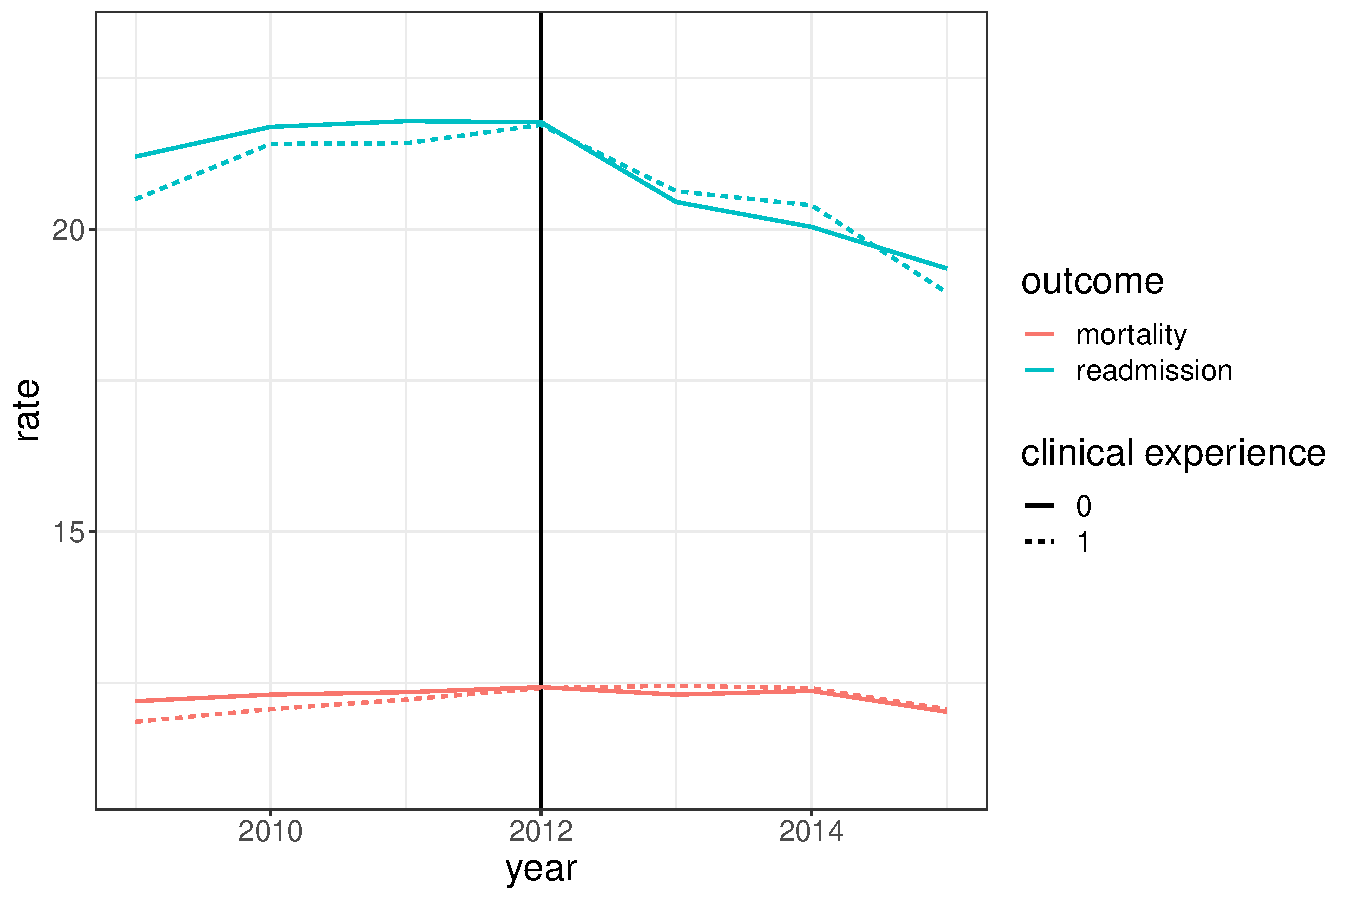
\includegraphics[scale=.6]{Objects/weighted_read_mort_graph.pdf}
        \label{weighted_read_mort_graph}
    \end{figure}

    \section{Model and Empirical Strategy}

    Not knowing the true form of nonprofit hospital objective functions, we can assume that they maximize some weighted average of revenue and quality. At a basic level, we can think of nonprofits behaving according to:     
    
    $$\max\hspace{2mm} \delta R + (1-\delta) u(\theta)$$

    \noindent where $R$ is net revenue, $u(.)$ is an increasing function that captures utility from quality of care, and $\theta$ is some quality of care measure. In this setting, we care about hospital responding to a penalty by adjusting readmission rates, so $\theta = 1-r$ where $r$ is the readmission rate. While previous research has set out to understand the average $\delta$ for nonprofit hospitals, $\delta$ may also be dependent on the leadership teams within nonprofit hospitals. Further, introducing the HRRP means that $R$ is directly dependent on $\theta$. We can then write the hospital's problem as 

    $$\max\hspace{2mm} \delta(L) R(\theta) + (1-\delta(L)) u(\theta)$$

    \noindent where $L$ captures the composition of the leadership team. Therefore, when maximizing this function, $\theta$ is dependent on $L$ through its impact on how the hospital values profit vs. quality of care.

    Thus, I directly estimate the effect of having clinical experience on readmission rates. However, looking purely at this correlation is likely a biased picture of the effect of clinical experience since it likely captures reverse causality: certain types of hospitals may be more likely to hire doctors as executives. I do two things to address this issue. First, as discussed in detail in Section \ref{sec:data}, I only consider hospitals with stable leadership teams over time. Second, I leverage the HRRP shock, limiting the sample to those that were penalized, which allows me to identify hospitals similar in quality along readmission rates, and to observe changes in behavior after the shock. For the hospitals in my sample, I define their type as having clinical experience on their executive team or not, a time invariant categorization. 

    I estimate the following regression equation:

    $$y_{ht} = \beta (clinical \times post\_penalty)_{ht} + \alpha_{h} + \delta_t + \epsilon_{ht}$$

    \noindent where $y_{ht}$ is one of the outcome variables discussed in Section \ref{sec:data}, $\beta$ is the variable of interest capturing the effect of having clinical experience after the penalties took place, $\alpha_h$ and $\delta_t$ are hospital and time fixed effects, respectively. 

    For identification, I rely on the assumption that, prior to being penalized, clinical and non-clinical team hospitals did not differentially change readmission rates for a reason I do not capture here. I investigate this assumption by estimating event study coefficients, where the coefficients $\beta_j$ now capture the effect of having clinical experience in a particular year, and $\beta_{2011}$ is normalized to zero:

    $$y_{ht} = \sum_{j=2009}^{2010}\beta_j(clinical_{ht} \times \mathbf{1}\{y=j\}) + \sum_{j=2012}^{2015}\beta_j (clinical_{ht} \times \mathbf{1}\{y=j\}) + \alpha_{h} + \delta_t + \epsilon_{ht}.$$


    \section{Results}

    \import{Tables}{read_results_table.tex}


    \begin{figure}
        \centering
        \caption{Event Study Estimates}
        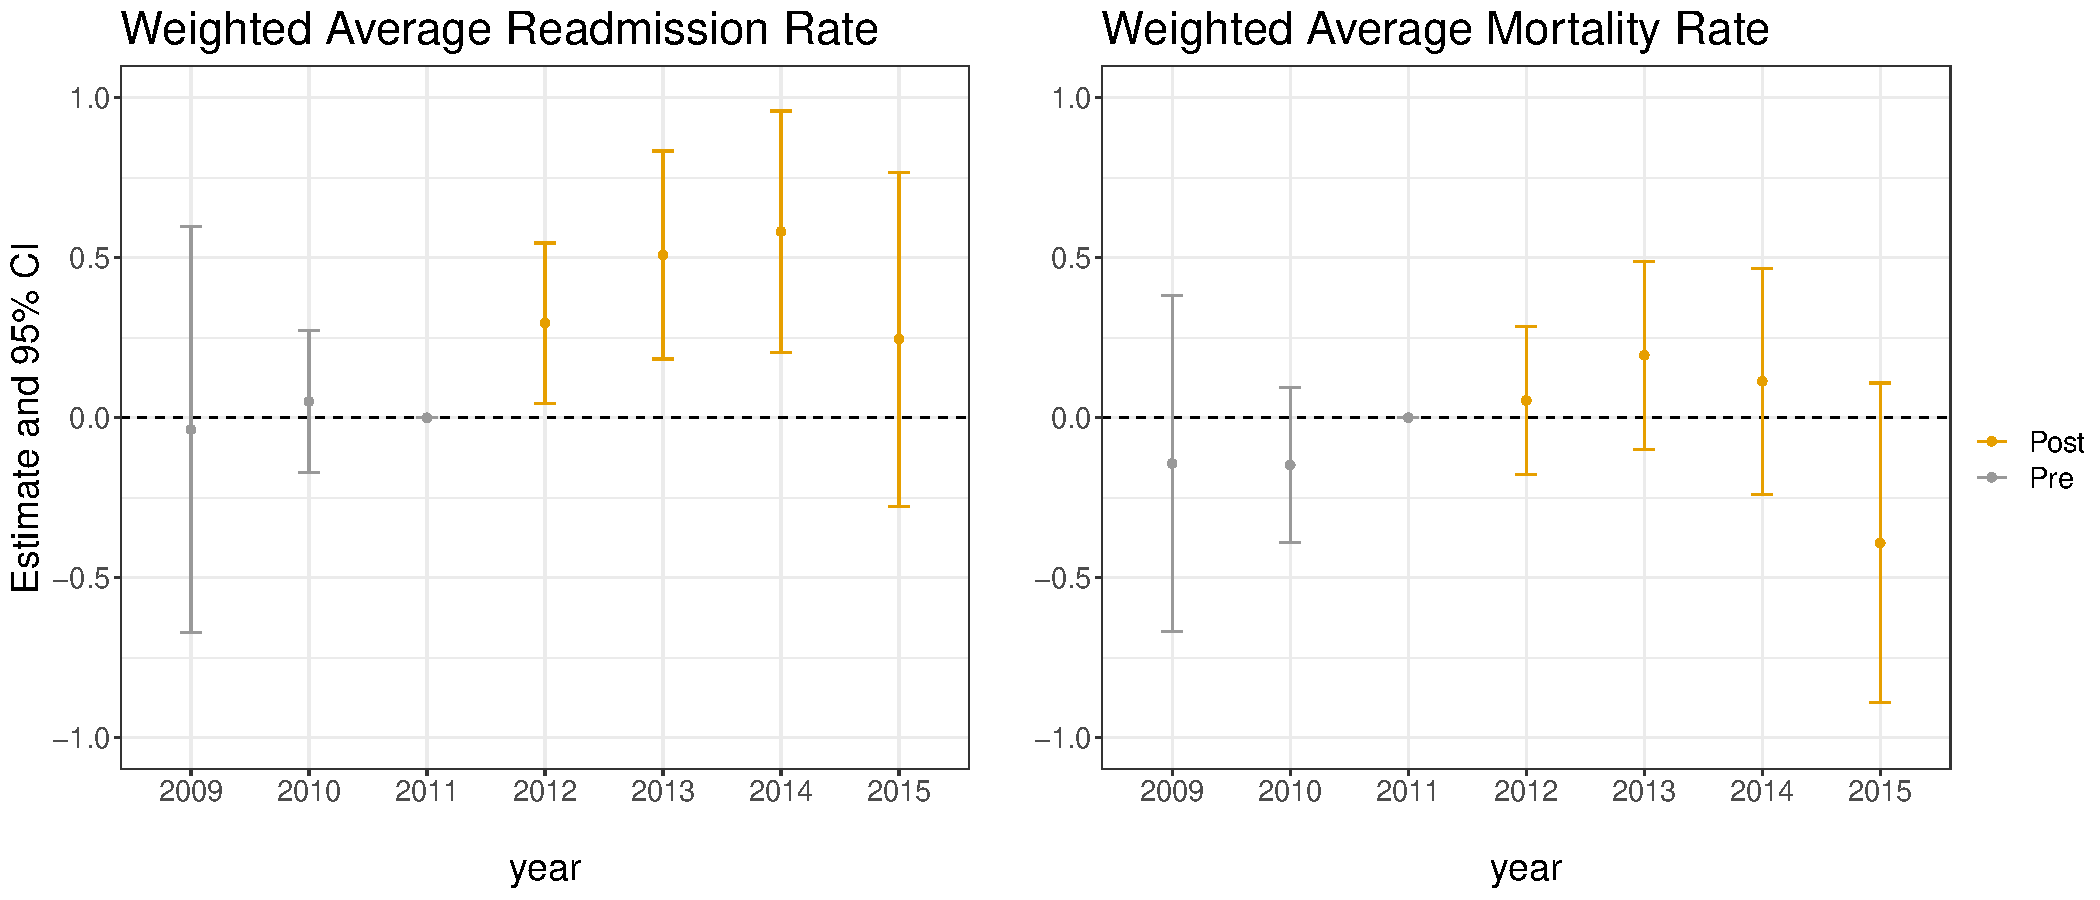
\includegraphics[scale=.5]{Objects/wa_eventstudy.pdf}
        \label{fig:wa_eventstudy}
    \end{figure}

    \section{Conclusion}

	
	\newpage
	\appendix

    \section{Data}\label{appendixdata}

    \subsection{Gathering Hospital Leadership Names}

    There is no perfect way to access tax form 990s in bulk over the time period I am considering in this paper. However, using the NonProfit Explorer API seems to be the most straightforward. At the time of writing this, information on using version 2 of the API can be found at \hyperlink{https://projects.propublica.org/nonprofits/api}{https://projects.propublica.org/nonprofits/api}. 
    
    There are over 1.5 million nonprofit entities in the US (cite), making it crucially important to be able to filter by type of entity before analyzing any PDFs. The API allows this by filtering a query based on National Taxonomy of Exempt Entities (NTEE) code. I query only nonprofits categorized as E20 (hospitals), E21 (community health systems), and E22 (general hospitals). The API has a pagination limit of 100, meaning I can only pull information on 100 hospitals at a time. Therefore, I filter the query further to only consider one state at a time. The only state that has more than 100 entities registered is California, and thus I subset the California query even further by names that include the word "hospital" and names that don't. I combine all of these subsets and have information on each nonprofits Employee Identification Number. There are 5,588 EINs total in this list. This acts as a list of entities for which I can pull more information. 

    I loop through the list of EINs found in the previous step and query more detailed information from the API on that specific EIN. I save the name, secondary name, state, and zip code, all of which do not vary by year. I also save each year's URL that links to the Tax Form 990 PDF. For the sake of a comprehensive data set, I keep years 2006-2020 (I later limit to 2009-2016 when focusing on the Hospital Readmissions Reduction Program). Thus, I finish this step with a panel data set of EIN characteristics and PDF locations. Importantly, there are multiple types of Tax Form 990s depending on the size of the nonprofit. In many cases, one nonprofit has at least two different forms filed in a given year. I filter out any EIN-years for which there are no PDFs on file. The data on PDF locations contains 4,012 EINs and 61,363 EIN-year-tax forms.

    It is crucial to the analysis to be able to link these nonprofits with other sources of data to recover penalties from HRRP, bed size, and outcomes of interest (definitely need to talk more about outcomes). Therefore, I take a conservative approach to matching EINs to American Hospital Association (AHA) ID, which links fairly easily to Medicare ID numbers, based on name and location. First, I will discuss limitations and cleaning that I do to the AHA data and tax form data separately before doing any matching. 

    I download the AHA data from Wharton Research Data Services. I filter only to hospitals in the contiguous US, Alaska, and Hawaii (excluding places like Puerto Rico), classified as nonprofit or state/community, and those that are general acute care. I also filter out any hospitals who weren't present in the data (or change system ID) in 2009-2015, meaning they either closed or were acquired. Due to the survey nature of this data, a hospital name may look slightly different from one year to the next. For example, "Waldo County General Hospital" is also Waldo County General Hospital Maine Health". Further, zip codes may change by one or two digits, making them unreliable to match based on. To deal with this, I first keep only unique AHA ID, name, zip, state, and system name combinations. Then, I convert the data from long to wide so that each AHA ID occurs only once, but may have multiple names, zip codes, or system names associated with it.

    I consider which nonprofit entities are not likely to be hospitals and drop them. There are numerous foundations or auxiliary nonprofits with the purpose of raising funds for the hospital, but do not actually care for patient. I filter out any nonprofit with "foundation" or "auxiliary" in the name. I also filter out various specialty centers that fell into the general hospital category, such as hospice or cancer centers. 

    I then proceed matching based on names in multiple layers. I focus on exact string matches, so I remove all spaces and common characters that could cause mismatches such as \&, ', -, and inc. Next, I take each AHA name and look for exact matches in a nonprofit's first or secondary name only for nonprofits in the same state as the AHA hospital. When an exact match is found, I record the link between AHA ID and EIN. In this first layer of matching, 860 hospitals in the AHA data are linked to an EIN, equivalent to 31\% of AHA nonprofit hospitals in the sample. 

    In the next layer of matching, I remove common words such as "healthcare", "regional", "hospital", etc. That way if there are subtle differences in names, removing common words may allow for an exact match. Again, I take each AHA hospital name and look for exact matches in the nonprofits within the same state. This adds an additional 90 hospital matches, accounting for a total of 34.5\% of AHA hospitals. 

    In some cases, tax forms are associated with a system of hospitals instead of one individual hospital. Thus, I create another variable that captures the names of systems which match. The process of matching is the same, the only difference is that now I am considering system names from the AHA data instead of hospital names. A total of 1,136 AHA hospitals have an EIN match on hospital name, system name, or both. This is roughly 41\% of the sample. These hospitals become the main sample for my analysis. While not capturing a large majority of AHA hospitals that are categorized as nonprofit, I would rather be conservative in selecting hospitals which I am confident that the characteristics and measurement of the independent and dependent variables are accurate. 

    (add a paragraph about validity of matches)

    Now that I have a sample of hospitals, the next step is to extract the names of the people in charge of these hospitals from the Tax Form 990 PDFs. In the data set of hospital PDF URLs that I collected earlier, I limit to the hospitals with solid matches described above. I then loop through each EIN, downloading each PDF locally and using tesseract package in R to extract text from the relevant pages of the PDF using OCR text extraction methods. In particular, I loop through each page of the PDF, look for the title associated with leadership names: ``Officers, Directors, Trustees, Key Employees, and Highest Compensated Employees", and save all the text from any pages where this title is found. I save the text to a list of all EIN, years present. 

    One tricky aspect of the NonProfit Explorer API is that, only in some cases, if two forms are present for an EIN, year, only the first one (which is typically not the one with the relevant information) is pulled. Therefore, for some hospitals, a couple years will have gaps in text extraction data. I locate EIN, years where this problem is occurring, and a team of RAs locates and downloads the correct forms manually. I extract text from these manually downloaded forms in the same manner as above. 

    The form of the text data is a data frame with one column, where each line of text is saved in a different row. I write a text cleaning package that locates names, positions, titles, and indications of resigning. I will now describe this function in three parts: preliminary cleaning of strings, locating names, and locating positions, titles, and key words surrounding resigning. 

    Typically on the same page as the names and positions is a list of the highest compensated employees and their compensation. In order to not record extra names, I filter out any rows after the start of this section. I then remove any digits, parentheses and brackets, other punctuation, letters that occur by themselves, two letter ``words" that have no meaning, and excess space between words. I then split up the phrase into individual words, so one phrase with 5 words is broken up into 5 variables. 

    Next, I locate first and last names in the data. 


    

    

    

    

    

    

	
	
	


\end{document}

